\documentclass[11pt]{beamer}
\usetheme{Berkeley}
\usepackage[utf8]{inputenc}
\usepackage[english]{babel}

\usepackage{amsmath,amsfonts,amssymb, nicefrac}
\usepackage{lmodern}
\usepackage{hyperref}
\usepackage{booktabs,array,ragged2e}
\usepackage{graphicx,subfigure}
\usepackage{fancyvrb}

\graphicspath{{./pics/}}

\usepackage{tikz}
\usetikzlibrary[decorations.pathmorphing]
\usetikzlibrary{mindmap}
\usetikzlibrary{graphs}

\usepackage{spverbatim}


%_______________________________________________________________________________
% Listings
%_______________________________________________________________________________
\usepackage{listings}
\usepackage{color}

\definecolor{mygreen}{rgb}{0,0.6,0}
\definecolor{mygray}{rgb}{0.5,0.5,0.5}
\definecolor{mymauve}{rgb}{0.58,0,0.82}

\lstset{
basicstyle=\footnotesize,        % the size of the fonts that are used for the code
breakatwhitespace=false,         % sets if automatic breaks should only happen at whitespace
breaklines=true,    
  commentstyle=\color{mygreen}, 
  frame=single,   
  keywordstyle=\color{blue}, 
  rulecolor=\color{black},
  stringstyle=\color{mymauve}}

%_______________________________________________________________________________
% Commands
%_______________________________________________________________________________
\newcommand{\R}{\mathbb{R}}
\newcommand{\C}{\mathbb{C}}
\newcommand{\N}{\mathbb{N}}
\newcommand{\Zn}{\mathbb{Z}^n_{\geq 0}}
\newcommand{\V}{\mathbf{V}}
\newcommand{\I}{\mathbf{I}}
\newcommand{\mvar}[2]{#1_1,\ldots , #1_{#2}}
\newcommand{\kxn}{k[\mvar{x}{n}]}
\newcommand{\fs}{\mvar{f}{s}}
%\newcommand{\mc}[1]{\boldsymbol{1}^{(#1)}}
\newcommand\mc[1]{{\vphantom{\bar{\boldsymbol{1}}}\boldsymbol{1}}^{\mkern-2mu (#1)}}
\newcommand{\mcb}[1]{\bar{\boldsymbol{1}}^{(#1)}}
\newcommand{\ya}{\mc{1}\mcb{4}\mc{6}}
\newcommand{\yb}{\mc{2}\mcb{3}\mc{5}}
\newcommand{\yc}{\mc{2}\mcb{4}\mc{6}}
\newcommand{\yd}{\mc{1}\mc{2}\mcb{6}}
\newcommand{\ye}{\mcb{3}\mc{4}\mc{6}}
\newcommand{\yf}{\mcb{5}\mc{6}}
\newcommand{\yfs}{\mcb{5}\mc{6}\mc{6}}


\author{Philipp Arras}
\title{Bachelor thesis}
\institute{Institute for Theoretical Physics Heidelberg} 
\begin{document}

\begin{frame}
\titlepage
\end{frame}

\begin{frame}
\tableofcontents
\end{frame}

\section{Mathematical Tools}
\subsection{Ideals and Varieties}
\begin{frame}{Ideals}
\textbf{Definition}
\begin{enumerate}
\item $0 \in I$.
\item $f,g\in I \;\Rightarrow \; f+g\in I$.
\item $f\in I$ and $h\in k[\mvar{x}{n}] \;\Rightarrow\; hf\in I$.
\end{enumerate}
$\Rightarrow\quad$ Set of consequences of $f_1 = \ldots = f_n = 0$. 

\begin{align*}
\langle \mvar{f}{s} \rangle := \left\lbrace \sum_{i=1}^s h_i f_i \; : \;  \mvar{h}{s} \in \kxn \right\rbrace
\end{align*}
\end{frame}

%\section{Old slides}
%\begin{frame}{Physical set-up}
\tikz
	\graph[grow down, branch right=5cm] {
		x1/"spacetime-filling D7-branes" -> {
			"spacetime-filling",
			"D7-branes"->"8 real dimensions"
		}-> x3/"4 real dimensions on $M^6$";
	};
\end{frame}
%\begin{frame}{Complex structure on $M^6$}
$\mathcal{N}=1$ SUSY leads to a  complex structure on $M^6$
\tikz
	\graph[grow down, branch right=5cm] {
		"spacetime filling 7-brane" -> "respects SUSY" -> "respects complex structure on $M^6$" -> "can be described as complex polynomial"
	};
\end{frame}
%\begin{frame}{Physical set-up}
\tikz
	\graph[grow down, branch right=5cm] {
		x1/"spacetime-filling D7-branes" -> {
			"spacetime-filling",
			"D7-branes"->"8 real dimensions"
		}-> x3/"4 real dimensions on $M^6$" -> "2 complex dimensions on $M^6$";
	};
\end{frame}
%\begin{frame}{$SU(N)$ gauge theory}
\begin{figure}
\centering
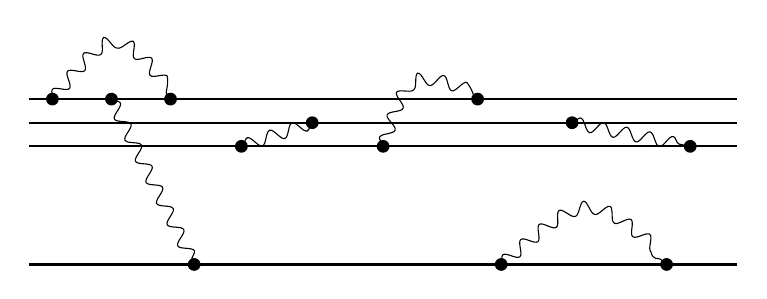
\begin{tikzpicture}[scale=0.3]
% horizontal lines
\draw[ thick] (0,9) -- (30,9);
\draw[ thick] (0,10) -- (30,10);
\draw[ thick] (0,11) -- (30,11);
\draw[ thick] (0,4) -- (30,4);
% strings
\filldraw (1,11) circle [radius=7pt];
\filldraw (6,11) circle [radius=7pt];
\draw[decorate,decoration={snake,amplitude=.8mm,segment length=3mm}] (1,11) .. controls (3.5,14) .. (6,11);
\filldraw (3.5,11) circle [radius=7pt];
\filldraw (7,4) circle [radius=7pt];
\draw[decorate,decoration={snake,amplitude=.8mm,segment length=3mm}] (3.5,11) -- (7,4);

\filldraw (15,9) circle [radius=7pt];
\filldraw (19,11) circle [radius=7pt];
\draw[decorate,decoration={snake,amplitude=.8mm,segment length=3mm}] (15,9) .. controls (16,12) .. (19,11);

\filldraw (23,10) circle [radius=7pt];
\filldraw (28,9) circle [radius=7pt];
\draw[decorate,decoration={snake,amplitude=.8mm,segment length=3mm}] (23,10) -- (28,9);

\filldraw (12,10) circle [radius=7pt];
\filldraw (9,9) circle [radius=7pt];
\draw[decorate,decoration={snake,amplitude=.8mm,segment length=3mm}] (12,10) -- (9,9);

\filldraw (20,4) circle [radius=7pt];
\filldraw (27,4) circle [radius=7pt];
\draw[decorate,decoration={snake,amplitude=.8mm,segment length=3mm}] (20,4) .. controls (23.5,7) .. (27,4);
\end{tikzpicture}
\end{figure}
$N$ D7-branes on top of each other give rise to $N^2$ vector states.
\end{frame}
%\begin{frame}{Intersection of 7-branes in F-theory}
\begin{figure}[h]
\centering
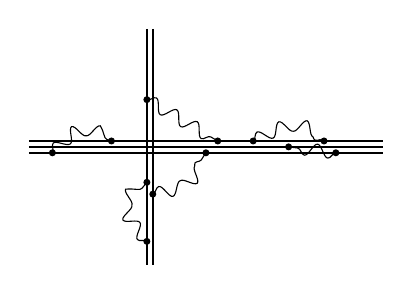
\begin{tikzpicture}[scale=.15]
% horizontal lines
\draw[ thick] (0,9.5) -- (30,9.5);
\draw[ thick] (0,10) -- (30,10);
\draw[ thick] (0,10.5) -- (30,10.5);
% vertical lines
\draw[ thick] (10,20) -- (10,0);
\draw[ thick] (10.5,20) -- (10.5,0);
% strings
\filldraw (10.5,6) circle [radius=7pt];
\filldraw (15,9.5) circle [radius=7pt];
\draw[decorate,decoration={snake,amplitude=.8mm,segment length=3mm}] (10.5,6) .. controls (13,6.5) .. (15,9.5);
\filldraw (10,14) circle [radius=7pt];
\filldraw (16,10.5) circle [radius=7pt];
\draw[decorate,decoration={snake,amplitude=.8mm,segment length=3mm}] (10,14) -- (16,10.5);

\filldraw (10,2) circle [radius=7pt];
\filldraw (10,7) circle [radius=7pt];
\draw[decorate,decoration={snake,amplitude=.8mm,segment length=3mm}] (10,2) .. controls (8,4.5) .. (10,7);

\filldraw (2,9.5) circle [radius=7pt];
\filldraw (7,10.5) circle [radius=7pt];
\draw[decorate,decoration={snake,amplitude=.8mm,segment length=3mm}] (2,9.5) .. controls (4,11.5) .. (7,10.5);

%\filldraw (5,9.5) circle [radius=7pt];
%\filldraw (9,9.5) circle [radius=7pt];
%\draw[decorate,decoration={snake,amplitude=.8mm,segment length=3mm}] (5,9.5) .. controls (7,8) .. (9,9.5);

\filldraw (19,10.5) circle [radius=7pt];
\filldraw (25,10.5) circle [radius=7pt];
\draw[decorate,decoration={snake,amplitude=.8mm,segment length=3mm}] (19,10.5) .. controls (22,12) .. (25,10.5);

\filldraw (26,9.5) circle [radius=7pt];
\filldraw (22,10) circle [radius=7pt];
\draw[decorate,decoration={snake,amplitude=.8mm,segment length=3mm}] (26,9.5) -- (22,10);
\end{tikzpicture}
\end{figure}
\begin{itemize}
\item[$\rightarrow$] In the intersection locus charged (anti-)chiral multiplets are localized.
\end{itemize}
\end{frame}

\begin{frame}{Overview geometric objects}
\begin{table}
\centering
\begin{tabular}{p{0.35\textwidth}|p{0.35\textwidth}|c}
Geometry&Physics&Dimension\\
\toprule
open strings on branes & gauge bosons & $\dim_{\C} = 2$\\\midrule
intersection of two branes & matter & $\dim_{\C} = 1$\\\midrule
intersection of two matter curves & interaction & $\dim_{\C} = 0$\\
\bottomrule
\end{tabular} 
\end{table}
\end{frame}
%\begin{frame}{Given objects}
\tikz
	\graph[grow down, branch right=5cm] {
		"elliptic fibration" -> "three 7-branes given as sets of polynomial equations" -> "Mathematical description in terms of \textbf{varieties}.";
	};


\emph{Example:}
\begin{align*}
0&=d_0 c_2^2 + b_0^2 c_1 - b_0 b_1 c_2\\
0&=d_1 b_0 c_2 - b_0^2 b_2-c_2^2 d_2
\end{align*}
\end{frame}
%\begin{frame}{Algebraic geometry}
%\tikz[grow cyclic, align=flush center,
%	level 1/.style={level distance=3 cm,sibling angle=90},
%	level 2/.style={level distance=2cm, sibling angle=30,font=\footnotesize , text width=2cm}]
\resizebox{!}{0.6\textwidth}{
\tikz[mindmap, grow cyclic, align=flush center,
	every node/.style={concept, execute at begin node=\hskip0pt},
	concept color=black!20,
	root concept/.append style={concept color=black, fill=white, line width=1em, text=black, font=\large\scshape},
	text=white,
	level 1/.style={level distance=6cm,sibling angle=90,font=\scshape},
	level 2/.style={level distance=6cm, sibling angle=60,font=\footnotesize , text width=2cm}]
	\node[root concept] {Algebraic geometry} %root
		child [concept color=red] { node {ideals}
			child { node {ideals generated by} }
			child { node {radical ideals} }
			child { node {prime ideals} }
			child { node {sum, product, intersection} }
		}
		child { node {varieties}
			child { node {$\V$} }
			child { node {$\I$} }
		}
		child { node {Zariski topology}
			child { node {Zariski closed $\Rightarrow$ standard closed} }
			child { node {not Hausdorff} }
			child { node {closure} }		
		}
		child {node {Decomposition of a variety}
			child { node {irreducible sets $\Leftrightarrow \I (V)$ prime } }
			child { node {$\exists$ a finite decomposition into irreducibles} }
			child { node {primary decomposition} }		
		};
}
\end{frame}

%%\begin{frame}{Test}
%\begin{tikzpicture}
%	[text width=2.7cm, align=flush center,grow cyclic,
%	level 1/.style={level distance=2.5cm,sibling angle=90},
%	level 2/.style={text width=2cm, font=\footnotesize, level distance=3cm,sibling angle=30}]]
%\node {asdfdfsd}
%   child { node {Computational Problems}
%      child { node {Problem Measures} }
%      child { node {Problem Aspects} }
%      child { node {Problem Domains} }
%      child { node {Key Problems} }
%    }
%    child { node {Computational Models}
%      child { node {Turing Machines} }
%      child { node {Random-Access Machines} }
%      child { node {Circuits} }
%      child { node {Binary Decision Diagrams} }
%      child { node {Oracle Machines} }
%      child { node {Programming in Logic} }
%    };
%\end{tikzpicture}
%sdf
%\end{frame}

\begin{frame}
\tikz
	\graph[grow down, branch right=5cm] {
		x1/"spacetime-filling D7-branes" -> {
			"spacetime-filling",
			"D7-branes"->"8 real dimensions"
		}-> x3/"4 real dimensions on $M^6$";
	};
\end{frame}




\end{document}